\subsection{Uspořádání}
\label{ssec:usporadani}

Uspořádání je poslední v jistém smyslu speciální relací, na kterou se podíváme.
Podobně jako ekvivalence, uspořádání mezi dvěma množinami nedává úplně smysl,
takže se po celou sekci budeme soustředit na relaci na množině.

Určitě nejznámějším typem uspořádání je relace \uv{menší nebo rovno} (ne\-bo
\uv{menší}, \uv{větší nebo rovno} atd., to je jedno), kterou jistě všichni
známe. Tohle je ten příklad uspořádání, který doporučujeme mít na paměti,
kdykoli se zdají obecné definice těžko stravitelnými.

Existuje ale samozřejmě spousta jiných druhů uspořádání s rozlišnými spektry
užitku. Uveďme například uspořádání dělitelností, zcela zásadní v elementární
teorii čísel, nebo lexikografické uspořádání, kterým se řadí slova ve slovnících
a encyklopediích a dá se použít i pro řazení polynomů (například v důkazu
slavného Gaussova algoritmu).

Ještě před definicí uspořádání se ale musíme zmínit o pro ni klíčové vlastnosti
relací.

\begin{definition}[Antisymetrická relace]
 Relace $R$ na množině $A$ se nazývá
 \begin{itemize}
  \item \textbf{antisymetrická}, pokud $(x,y) \in R \Rightarrow (y,x) \notin R$
   pro všechny prvky ${x,y \in A}$.
  \item \textbf{slabě antisymetrická}, pokud $xRy \wedge yRx \Rightarrow x=y$ 
   pro všechna $x,y \in A$.
 \end{itemize}
\end{definition}

Jak název napovídá, vlastnost antisymetrie je opravdu jakýmsi protikladem
symetrie.

Přeložena do jazyka aspoň některých lidí, relace je (silně) antisymetrická
tehdy, když to, že je prvek $x$ v relaci s prvkem $y$, zakazuje, aby byl zároveň
$y$ v relaci s $x$. Může se však samozřejmě stát, že $x$ není v relaci s $y$ ani
$y$ není v relaci s $x$. Všimněte si, že vlastnost antisymetrie mimo jiné
\emph{nedovoluje, aby daná relace byla reflexivní}.

\begin{example}
 Všeobecně oblíbených příkladem (silně) antisymetrické relace je relace $<$,
 třeba na množině $\R$. V moment, kdy pro dvě reálná čísla $x,y \in \R$ platí,
 že $x<y$, pak automaticky \textbf{nemůže platit} $y<x$. Zároveň, žádné reálné
 číslo není nikdy ostře menší než ono samo, tedy $<$ je vskutku antisymetrická a
 není reflexivní.
\end{example}

Ačkoliv to možná z definice není zřejmé, vlastnost \emph{slabé} antisymetrie je
opravdu jen oslabená vlastnost (silné) antisymetrie v tom smyslu, že slabě
antisymetrická relace může být reflexivní. Čili, mám-li slabě antisymetrickou
relaci $R$, pak $xRy$ nutně \textbf{nezakazuje}, aby $yRx$, ale jediný prvek
$y$, pro který tato situace může nastat, je $x$ samotné.

\begin{example}
 Asi tušíte, co přijde. Když vám řekneme, abyste zeslabi\-li vztah $<$, prvním
 takovým přirozeným nápadem je vztah $ \leq $, což je skutečně slabě
 antisymetrická relace. Vskutku, když $x \leq y$, pak se může stát, že i $y \leq
 x$, ale to nutně znamená, že $x = y$.
\end{example}

\begin{definition}[Uspořádání]
 Relace $R$ na množině $A$ se nazývá
 \begin{itemize}
  \item (neostré) \textbf{uspořádání}, pokud je \emph{reflexivní}, \emph{slabě
   antisymetrická} a \emph{transitivní}.
  \item \textbf{ostré uspořádání}, pokud je \emph{antisymetrická} a
   \emph{transitivní}.
 \end{itemize}
 Pokud je $R$ (ostré) uspořádání na $A$, nazýváme dvojici $(A,R)$ (ostře)
 \textbf{uspořádanou množinou}.
\end{definition}

\begin{example}
 \hfill
 \vspace*{-.5\parskip}
 \begin{enumerate}
  \item Relace $<$ na $\R$ je \textbf{ostré uspořádání}, protože
   \begin{itemize}
    \item (antisymetrie) $x < y \Rightarrow y \nless x$ a
    \item (transitivita) $x < y \wedge y < z \Rightarrow x < z$
   \end{itemize}
   pro všechna čísla $x,y,z \in \R$.
  \item Relace $ \leq $ na $\R$ je (neostré) \textbf{uspořádání}. Vskutku, platí
   \begin{itemize}
    \item (reflexivita) $x \leq x$,
    \item (slabá antisymetrie) $x \leq y \wedge y \leq x \Rightarrow x = y$ a
    \item (transitivita) $x \leq y \wedge y \leq z \Rightarrow x \leq z$
   \end{itemize}
   pro všechna $x,y,z \in \R$.
 \end{enumerate}
\end{example}

Ještě poslední sousto nomenklatury.

\begin{definition}[Lineární uspořádání]
 (Ostré) uspořádání $R$ na množině $A$ nazveme \textbf{lineárním}, pokud pro každé dva
 prvky $x,y \in A$ platí, že $xRy$ nebo $yRx$. Čili, každé dva prvky $A$ spolu
 \emph{lze porovnat} prostřednictvím $R$. (Ostré) uspořádání, které \emph{není
 lineární}, často označujeme jako \textbf{částečné}.
\end{definition}

\begin{example}
 Jak $<$, tak $ \leq $, jsou lineární uspořádání.
\end{example}

Protože základní idea za pojmem \uv{uspořádání} je, no, uspořádání prvků na
množině, ujaly se pro jejich kreslení, spíše než mříže nebo šipky, tzv.
\emph{Hasseho diagramy}. Hasseho diagram vypadá tak, že prvky množiny jsou
značeny tečkami a mezi porovnatelnými prvky (tj. prvky, které jsou v relaci) se
dá dostat po úsečkách (někdy přes více prvků). Navíc, prvky se kreslí zezdola
nahoru vzhledem k jejich pozici v rámci daného uspořádání.

\begin{example}[Uspořádání velikostí]
 Již jsme zpozorovali, že $ \leq $ je uspořádání. Jeho Hasseho diagram na
 množině $\clr{A \coloneqq \{1,2,3,4,5\}}$ vidíte na
 \hyperref[fig:hasse-linear]{obrázku~\ref*{fig:hasse-linear}}.
 \begin{figure}[H]
  \centering
  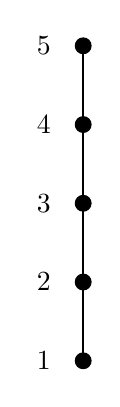
\begin{tikzpicture}
   \foreach \y in {1, 2, 3, 4, 5} {
    \node[circle,draw,fill=black,minimum size=2mm,inner sep=0pt,outer
    sep=0pt] at (0, \y - 1) {};
    \node at (-0.5, \y - 1) {$\clr{\y}$};
   }
   \foreach \y in {1, 2, 3, 4} {
    \draw[thick] (0, \y - 1) -- (0, \y);
   }
  \end{tikzpicture}
  \caption{Hasseho diagram uspořádáné množiny $(\clr{A}, \leq)$.}
  \label{fig:hasse-linear}
 \end{figure}
 Ve skutečnosti, Hasseho diagram \textbf{každého} lineárního uspořádání vypadá
 takto; liší se pouze počet prvků. Detaily si rozmyslíte za cvičení.
\end{example}

\begin{definition}[Dělitelnost]
 \label{def:delitelnost}
 Mějme čísla $m,n \in \N$. Říkáme, že $m$ \textbf{dělí} $n$, když existuje
 přirozené číslo $k \in \N$ takové, že $n = km$. Tento fakt zapisujeme jako $m
 \mid n$.
\end{definition}

\begin{example}[Uspořádání dělitelností]
 Relace $ \mid $ z \hyperref[def:delitelnost]{definice dělitelnosti} je ve
 skutečnosti uspořádání (důkaz jako cvičení), které \textbf{ale není lineární}.
 Jeho \hyperref[fig:hasse-delitelnost]{Hasseho diagram} na množině $\clr{A}
 \coloneqq \clr{[10]}$ je výrazně košatější.
 \begin{figure}[H]
  \centering
  \begin{tikzpicture}
   \node[circle,draw,fill=black,minimum size=2mm,inner sep=0pt,outer
   sep=0pt] (1) at (0, 0) {};
   \node[below=1mm of 1] {$\clr{1}$};

   \node[circle,draw,fill=black,minimum size=2mm,inner sep=0pt,outer
   sep=0pt] (2) at (-3, 1) {};
   \node[left=1mm of 2] {$\clr{2}$};

   \node[circle,draw,fill=black,minimum size=2mm,inner sep=0pt,outer
   sep=0pt] (3) at (-1, 1) {};
   \node[left=1mm of 3] {$\clr{3}$};

   \node[circle,draw,fill=black,minimum size=2mm,inner sep=0pt,outer
   sep=0pt] (5) at (1, 1) {};
   \node[right=1mm of 5] {$\clr{5}$};

   \node[circle,draw,fill=black,minimum size=2mm,inner sep=0pt,outer
   sep=0pt] (7) at (3, 1) {};
   \node[right=1mm of 7] {$\clr{7}$};

   \draw[thick] (1) -- (2);
   \draw[thick] (1) -- (3);
   \draw[thick] (1) -- (5);
   \draw[thick] (1) -- (7);

   \node[circle,draw,fill=black,minimum size=2mm,inner sep=0pt,outer
   sep=0pt] (4) at (-3, 2) {};
   \node[left=1mm of 4] {$\clr{4}$};

   \node[circle,draw,fill=black,minimum size=2mm,inner sep=0pt,outer
   sep=0pt] (8) at (-3, 3) {};
   \node[left=1mm of 8] {$\clr{8}$};

   \draw[thick] (2) -- (4);
   \draw[thick] (4) -- (8);

   \node[circle,draw,fill=black,minimum size=2mm,inner sep=0pt,outer
   sep=0pt] (8) at (-3, 3) {};
   \node[left=1mm of 8] {$\clr{8}$};

   \node[circle,draw,fill=black,minimum size=2mm,inner sep=0pt,outer
   sep=0pt] (6) at (-2, 2) {};
   \draw[thick] (2) -- (6);
   \draw[thick] (3) -- (6);
   \node[left=1mm of 6] {$\clr{6}$};

   \node[circle,draw,fill=black,minimum size=2mm,inner sep=0pt,outer
   sep=0pt] (9) at (-1, 2) {};
   \draw[thick] (3) -- (9);
   \node[right=1mm of 9] {$\clr{9}$};

   \node[circle,draw,fill=black,minimum size=2mm,inner sep=0pt,outer
   sep=0pt] (10) at (1, 2) {};
   \node[right=1mm of 10] {$\clr{10}$};
   \draw[thick] (2) -- (10);
   \draw[thick] (5) -- (10);
  \end{tikzpicture}
  \caption{Hasseho diagram uspořádané množiny $(\clr{A}, \mid)$.}
  \label{fig:hasse-delitelnost}
 \end{figure}
\end{example}

Lexikografické uspořádání je v principu uspořádání na slovech, ale může být
úspěšně použito třeba i pro uspořádání polynomů více proměnných. Funguje
následovně: slovem délky $n$ nazveme posloupnost $a_1a_2\ldots a_n$, kde $a_i$
je libovolné písmeno mezi \uv{a} a \uv{z}. Slovo $a_1a_2\ldots a_n$ je
lexikograficky níž než slovo $b_1b_2\ldots b_m$, pokud existuje $i \leq
\min(n,m)$ takové, že $a_1 = b_1 \wedge a_2 = b_2 \wedge \ldots \wedge a_{i-1} =
b_{i-1}$ a $b_i > a_i$.

Řečeno lidsky, o slově $a_1a_2\ldots a_n$ řeknu, že je níž než $b_1b_2\ldots
b_m$, když nějaké jeho písmeno $a_i$ je dřív v abecedě než písmeno $b_i$ na
stejném místě ve slově $b_1b_2\ldots b_m$. Pokud je jedno slovo plně součástí
druhého, lexikograficky níž je to kratší. Lexikografické uspořádání se obvykle
značí rovněž $ \leq $, ale pro přehlednost ho budeme značit třeba
$\leq_{\text{lex}}$.

\begin{example}[Lexikografické uspořádání]
 Jak si můžete ověřit (ale cvičení to nutně není), lexikografické uspořádání je
 lineární, takže jeho Hasseho diagram není dvakrát zajímavý. Pro úplnost zde
 ale přesto ukážeme \hyperref[fig:hasse-lex]{diagram} množiny
 \[
  \clr{A} \coloneqq \clr{\{a_1a_2 \mid a_i \in \{a,b,c\}\}},
 \]
 tedy množiny všech dvojpísmenných kombinací písmen \uv{a} až \uv{c}.
 \begin{figure}[H]
  \centering
  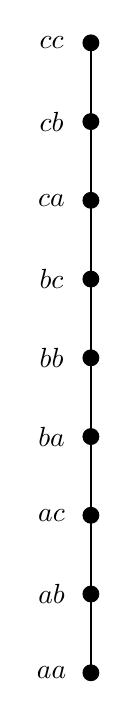
\begin{tikzpicture}
   \foreach \y in {1, 2, 3, 4, 5, 6, 7, 8, 9} {
    \node[circle,draw,fill=black,minimum size=2mm,inner sep=0pt,outer
    sep=0pt] at (0, \y - 1) {};
   }
   \foreach \y in {1, 2, 3, 4, 5, 6, 7, 8} {
    \draw[thick] (0, \y - 1) -- (0, \y);
   }
   \node at (-0.5, 0) {$\clr{aa}$};
   \node at (-0.5, 1) {$\clr{ab}$};
   \node at (-0.5, 2) {$\clr{ac}$};
   \node at (-0.5, 3) {$\clr{ba}$};
   \node at (-0.5, 4) {$\clr{bb}$};
   \node at (-0.5, 5) {$\clr{bc}$};
   \node at (-0.5, 6) {$\clr{ca}$};
   \node at (-0.5, 7) {$\clr{cb}$};
   \node at (-0.5, 8) {$\clr{cc}$};
  \end{tikzpicture}
  \caption{Hasseho diagram uspořádané množiny $(\clr{A}, \leq_{\text{lex}})$.}
  \label{fig:hasse-lex}
 \end{figure}
\end{example}

Velmi pěkné obrázky uspořádání vznikají i na množině všech množin $A$, tedy na
$2^{A}$, kde uspořádání je inkluzí $ \subseteq $. Tedy, nejníž je prázdná
množina, která leží uvnitř každé množiny, a nejvýš je množina $A$, ve které je
obsažena každá její podmnožina. Jeden malý příklad tu nakreslíme, určitě se vám
bude líbit.

\begin{example}
 Mějme množinu $A \coloneqq \{1,2,3\}$. Množinu $\clr{2^{A}}$ uspořádáme
 inkluzí, čili dvě podmnožiny $A$ jsou v relaci inkluze, když je jedna obsažena
 v druhé. Jeden příklad za všechny je třeba $\{1\} \subseteq \{1,3\}$.
 \hyperref[fig:hasse-power-set]{Hasseho diagram} takového uspořádání vidíte
 níže. V rámci úspory píšeme třeba $12$ místo množiny $\{1,2\}$.
 \begin{figure}[H]
  \centering
  \begin{tikzpicture}
   \node[circle,draw,fill=black,minimum size=2mm,inner sep=0pt,outer
   sep=0pt] (0) at (0, 0) {};
   \node[circle,draw,fill=black,minimum size=2mm,inner sep=0pt,outer
   sep=0pt] (1) at (-2, 2) {};
   \node[circle,draw,fill=black,minimum size=2mm,inner sep=0pt,outer
   sep=0pt] (2) at (0, 2) {};
   \node[circle,draw,fill=black,minimum size=2mm,inner sep=0pt,outer
   sep=0pt] (3) at (2, 2) {};
   \node[circle,draw,fill=black,minimum size=2mm,inner sep=0pt,outer
   sep=0pt] (12) at (-2, 4) {};
   \node[circle,draw,fill=black,minimum size=2mm,inner sep=0pt,outer
   sep=0pt] (13) at (0, 4) {};
   \node[circle,draw,fill=black,minimum size=2mm,inner sep=0pt,outer
   sep=0pt] (23) at (2, 4) {};
   \node[circle,draw,fill=black,minimum size=2mm,inner sep=0pt,outer
   sep=0pt] (123) at (0, 6) {};

   \draw[thick] (0) -- (1);
   \draw[thick] (0) -- (2);
   \draw[thick] (0) -- (3);
   \draw[thick] (1) -- (12);
   \draw[thick] (1) -- (13);
   \draw[thick] (2) -- (12);
   \draw[thick] (2) -- (23);
   \draw[thick] (3) -- (13);
   \draw[thick] (3) -- (23);
   \draw[thick] (12) -- (123);
   \draw[thick] (13) -- (123);
   \draw[thick] (23) -- (123);

   \node[below=1mm of 0]{$\clr{\emptyset}$};
   \node[left=1mm of 1]{$\clr{1}$};
   \node[left=1mm of 2]{$\clr{2}$};
   \node[right=1mm of 3]{$\clr{3}$};
   \node[left=1mm of 12]{$\clr{12}$};
   \node[left=1mm of 13]{$\clr{13}$};
   \node[right=1mm of 23]{$\clr{23}$};
   \node[above=1mm of 123]{$\clr{123}$};
  \end{tikzpicture}
  \caption{Hasseho diagram uspořádané množiny $(\clr{2^{A}}, \subseteq)$.}
  \label{fig:hasse-power-set}
 \end{figure}
\end{example}
Jako obvykle následuje několik cvičení na závěr sekce.

\begin{exercise}
 Udělejte cvičení rozmístěná po sekci. Konkrétně,
 \begin{enumerate}
  \item dokažte, že Hasseho diagram každého lineárního uspořádání má stejný tvar
   jako diagram na \hyperref[fig:hasse-linear]{obrázku~\ref*{fig:hasse-linear}}.
  \item dokažte, že relace dělitelnosti $ \mid $ je uspořádání na každé
   podmnožině přirozených čísel.
 \end{enumerate}
\end{exercise}

\begin{exercise}
 Explicitně popište všechny relace (na libovolné množině), které jsou zároveň
 ekvivalencí a (částečným) uspořádáním.
\end{exercise}

\begin{exercise}
 Řekněme, že $R$ a $S$ jsou uspořádání na množině $A$. Které z následujících
 relací jsou také uspořádáními na $A$?
  \begin{itemize}[itemsep=0pt]
  \item $R \cap S$ 
  \item $R \cup S$ 
  \item $R \setminus S$
  \item $R \circ S$
 \end{itemize}
\end{exercise}
